% --------------------------------------------------------------------------- %
% --------------------------------------------------------------------------- %
\section{Signal Interpretations}
\label{sec:interpretations}

The results of the search can be interpreted as a constraint on the mass of hypothesized particles of various BSM models. Based on the simulated production processes of simplified SUSY models, this section describes some of the uncertainties associated with the signal yield, as well as the limits associated with various simplified models of interest.

\subsection{Signal Yield Systematic Uncertainties}
\label{subsec:signalSyst}

The uncertainties associated with the signal yield are summarized in table \ref{tbl:signalSyst}. The various sources of uncertainty are described in detail below:
\begin{itemize}
	\item {\it Luminosity:} the uncertainty of the total integrated luminosity delivered by the LHC is evaluated in {\it Van Der Meer scans}, where the rate of interactions is measured while scanning the colliding proton beams across each other. The uncertainty in the luminosity based on these studies is 2.5\%.
	\item {\it Simulation statistics:} the limited size of the Monte Carlo samples for each sample effect the statistics in each signal region bin. After applying the signal selection, the statistical uncertainty can range from 1-100\% in different bins, though bins with large uncertainty typically correspond to those with low signal acceptance, and thus do not drive the sensitivity of the analysis to that simplified model mass point.
	\item {\it Renormalization and factorization scales:} the overall effect of varying the simulation renormalization and factorization scales of the underlying physics processes (and subsequent effect on event kinematics) is computed separately in each bin. The result of this variation is relatively flat and minor across the signal bins, and is conservatively estimated at 5\% for all regions.
	\item {\it Initial-state radiation (ISR) recoil:} variations of the boost due to initial-state radiation are performed to test the modeling of ISR effects in simulation. The effect of these variations ranges from 0-30\% across signal regions.
	\item {\it b-tagging efficiency:} the effect of varying the b-tag scale factor efficiency is calculated in each bin, and taken as a correlated error amongst all bins. The effect of this variation for heavy (light) flavor jets is 0-40\% (0-20\%) across signal regions.
	\item {\it Lepton efficiency:} the effect of varying the electron and muon scale factors applied to simulation is calculated in each bin, and taken as a correlated error amongst all bins. The effect of this variation is 0-20\% across signal regions.
	\item {\it Jet energy scale:} the effect of varying the jet energy scales is calculated in each bin, and the results are compatible with statistical uncertainty for low-statistics bins. Based on findings in the high-statistics bins, the uncertainty is estimated at 5\% for all regions.
	\item {\it Fast simulation modeling:} The signal Monte Carlo samples are generated using the FastSim package, which may result in modeling differences compared to Fullsim MC. Studies of the Fastsim kinematics with respect to \MET and pile-up modeling indicate differences of up to 5\% in some signal regions.
\end{itemize}

\begin{table}
	\centering
	\begin{tabular}[]{l c r}
		\fm{Summary table of signal systematics} 
	\end{tabular}
	\caption{Typical values of the systematic uncertainties associated with the simplified SUSY model signal yield for each interpretation in this search. Some systematics are taken as correlated amongst all signal regions; the rest are uncorrelated everywhere. Note that the large range of statistical uncertainty is driven by a small number of signal regions with low acceptance (which are not typically sensitive to those model points).}
	\label{tbl:signalSyst}
\end{table}

\subsection{Exclusion Limits}
\label{subsec:exclusionLimits}

The final results are interpreted in the context of various simplified SUSY models: gluino-mediated squark pair production, direct production of squarks, and alternative models of top squark production with different decay modes. Each of these models is illustrated in figure \ref{fig:signalFeynman}. For each pair producing gluino (squark) scenario, the models assume all SUSY particles other than the gluino (squark) and lightest neutralino are too massive to be produced directly and the gluino (squark) decays promptly. In addition, each model assumes that the gluino (squark) decays with a 100\% branching fraction into the decay products depicted in figure \ref{fig:signalFeynman}, except for models where the decays of the two squarks differ where a 50\% branching fraction for each decay mode is assumed. When considering top squark pair production, the polarization of the top quark is model dependent (and a function of the top-squark and neutralino mixing matrices), so events are generated without polarization to remain model-independent.
\begin{figure}
	\centering
	
\includegraphics[width=0.30\textwidth]{figs/placeholder}
	
\includegraphics[width=0.30\textwidth]{figs/placeholder}
	
\includegraphics[width=0.30\textwidth]{figs/placeholder}
	
\includegraphics[width=0.30\textwidth]{figs/placeholder}
	
\includegraphics[width=0.30\textwidth]{figs/placeholder}
	
\includegraphics[width=0.30\textwidth]{figs/placeholder}
	
\includegraphics[width=0.30\textwidth]{figs/placeholder}
	
\includegraphics[width=0.30\textwidth]{figs/placeholder}
	
\includegraphics[width=0.30\textwidth]{figs/placeholder}
	\caption{Feynman diagams depicting the different simplified SUSY models considered in this analysis. Results are interpreted in the context of gluino-mediated bottom, top, and light-flavor squark production (top), direct production of bottom, top, and light-flavor squarks (middle), and alternate decay modes of direct top squark production (bottom).}
	\label{fig:signalFeynman}
\end{figure}

The cross-section exclusion limits are calculated at 95\% confidence level (CL) for each simplified model. The limits are obtained using the background-fitting procedure described in section \ref{sec:yields} obtained with the higgsCombine tool. The 95\% CL exclusion limits for gluino-mediated models is shown in figure \ref{fig:limitsGluino}, for direct squark production in figure \ref{fig:limitsSquark}, and for alternate top squark decay modes in figure \ref{limitsStop}. The constraints on the masses of SUSY particles excluded by this search is summarized in table \ref{tbl:limits}.
\begin{figure}
	\centering
	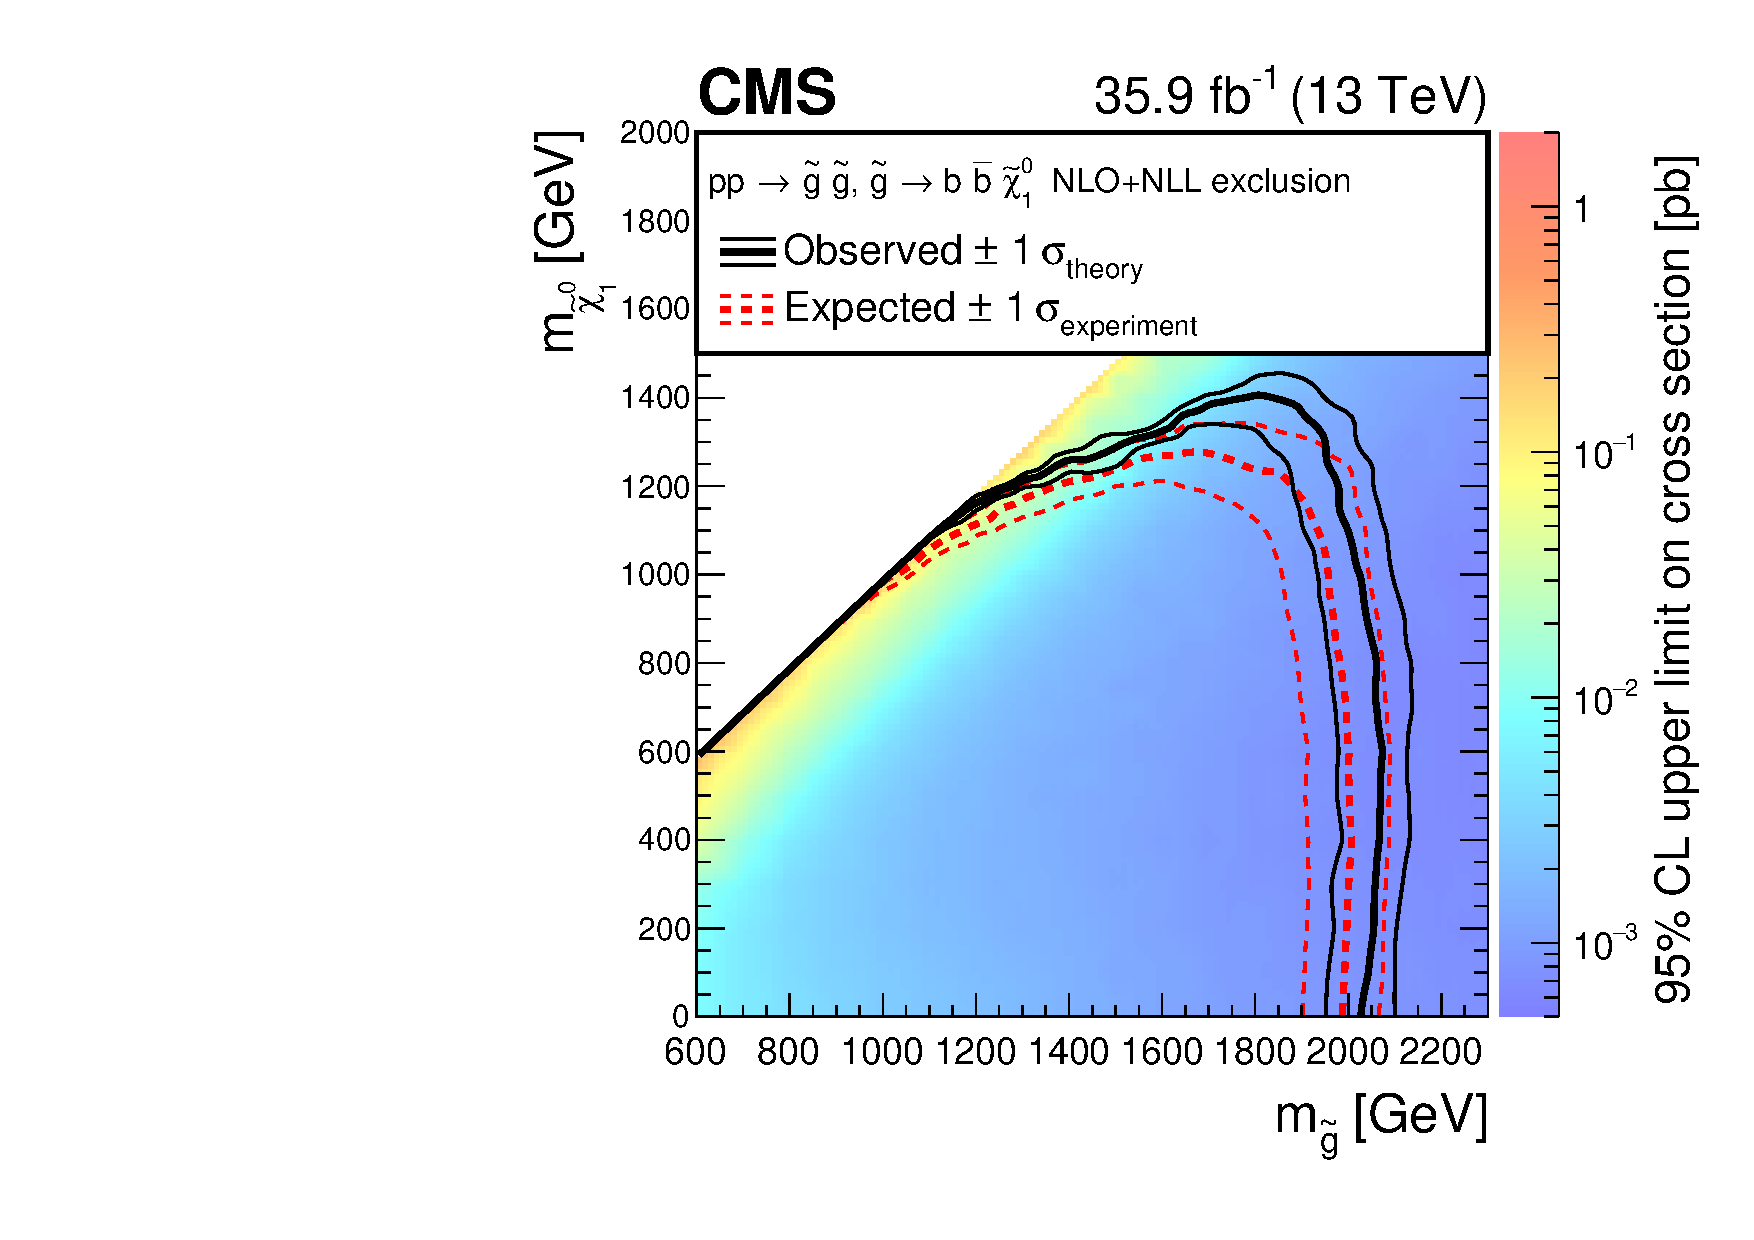
\includegraphics[width=0.45\textwidth]{results/figs/interpretations/T1bbbb_35p9ifb_Moriond2017_Mar07_XSEC}
	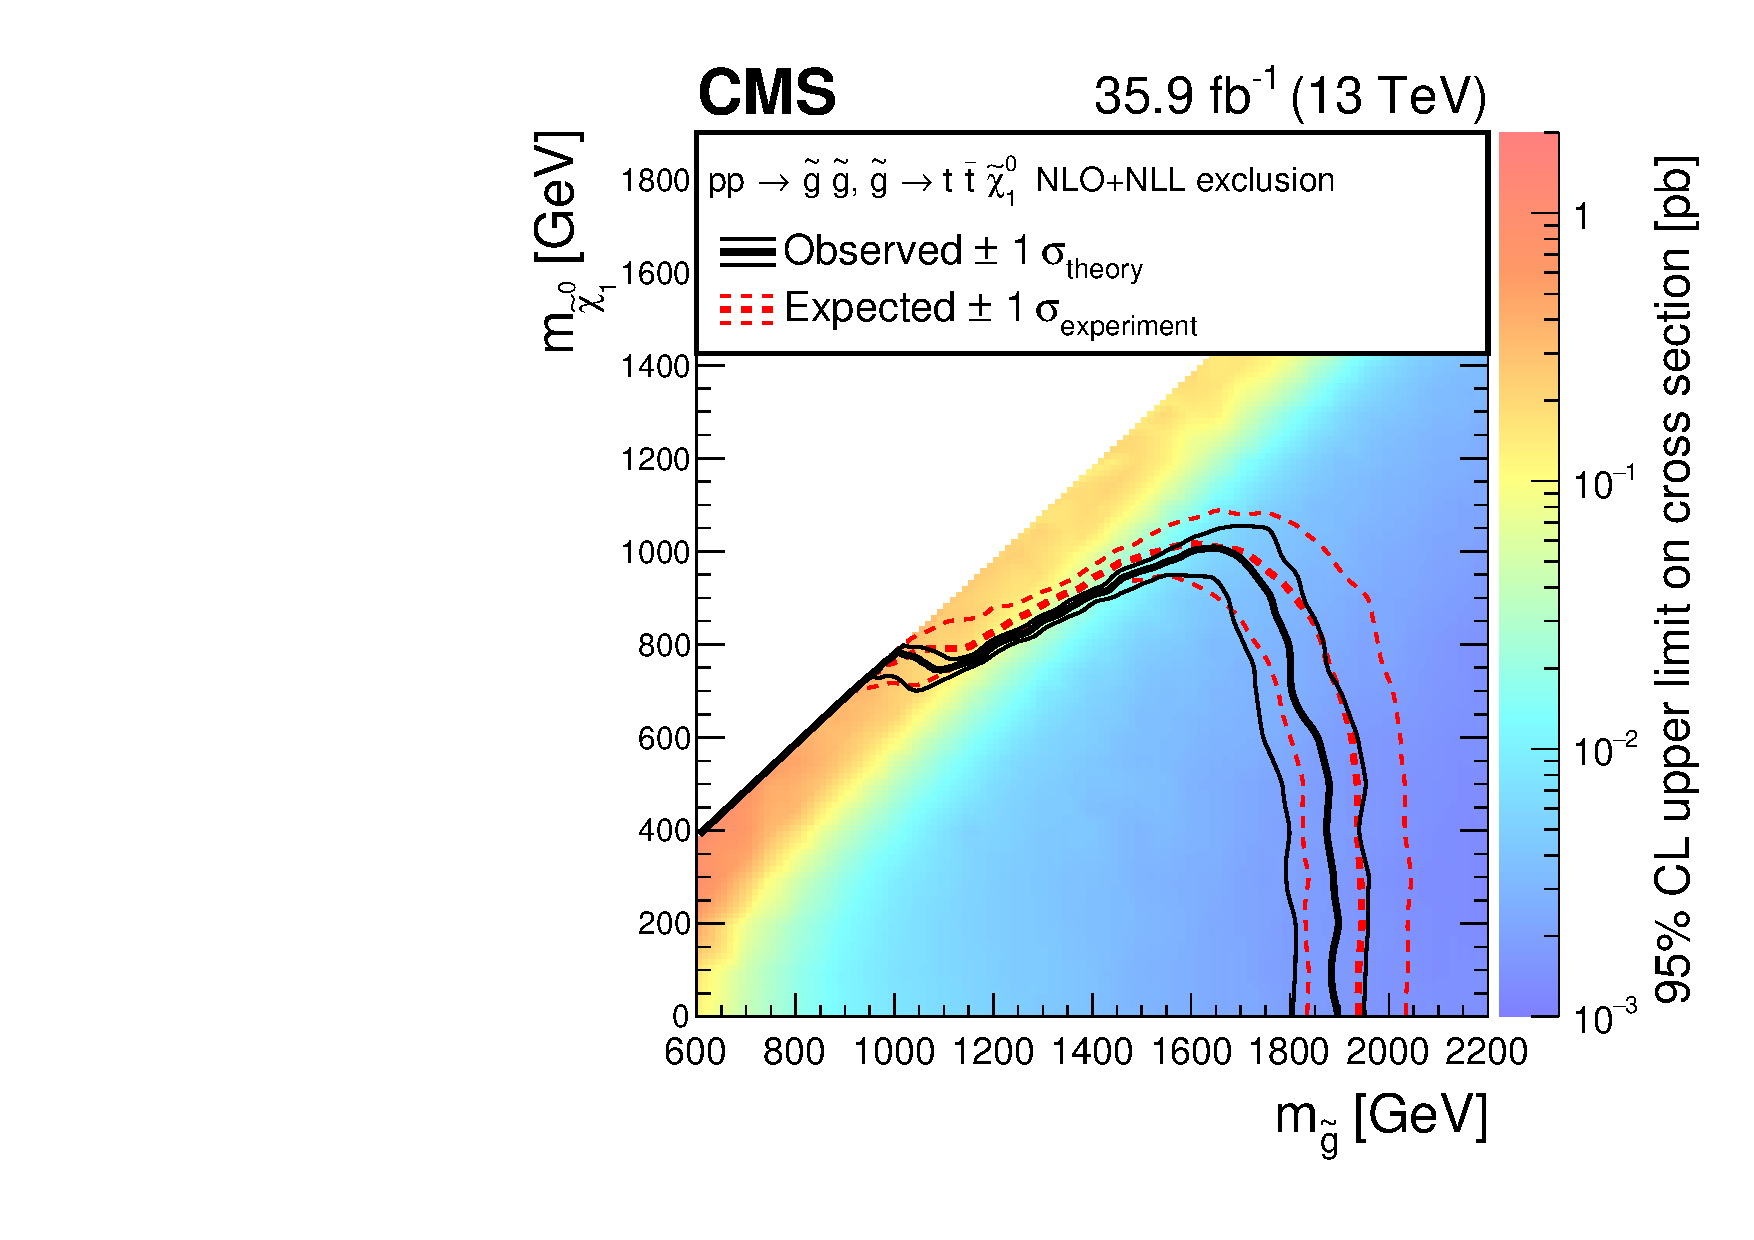
\includegraphics[width=0.45\textwidth]{results/figs/interpretations/T1tttt_35p9ifb_Moriond2017_Mar07_XSEC}
	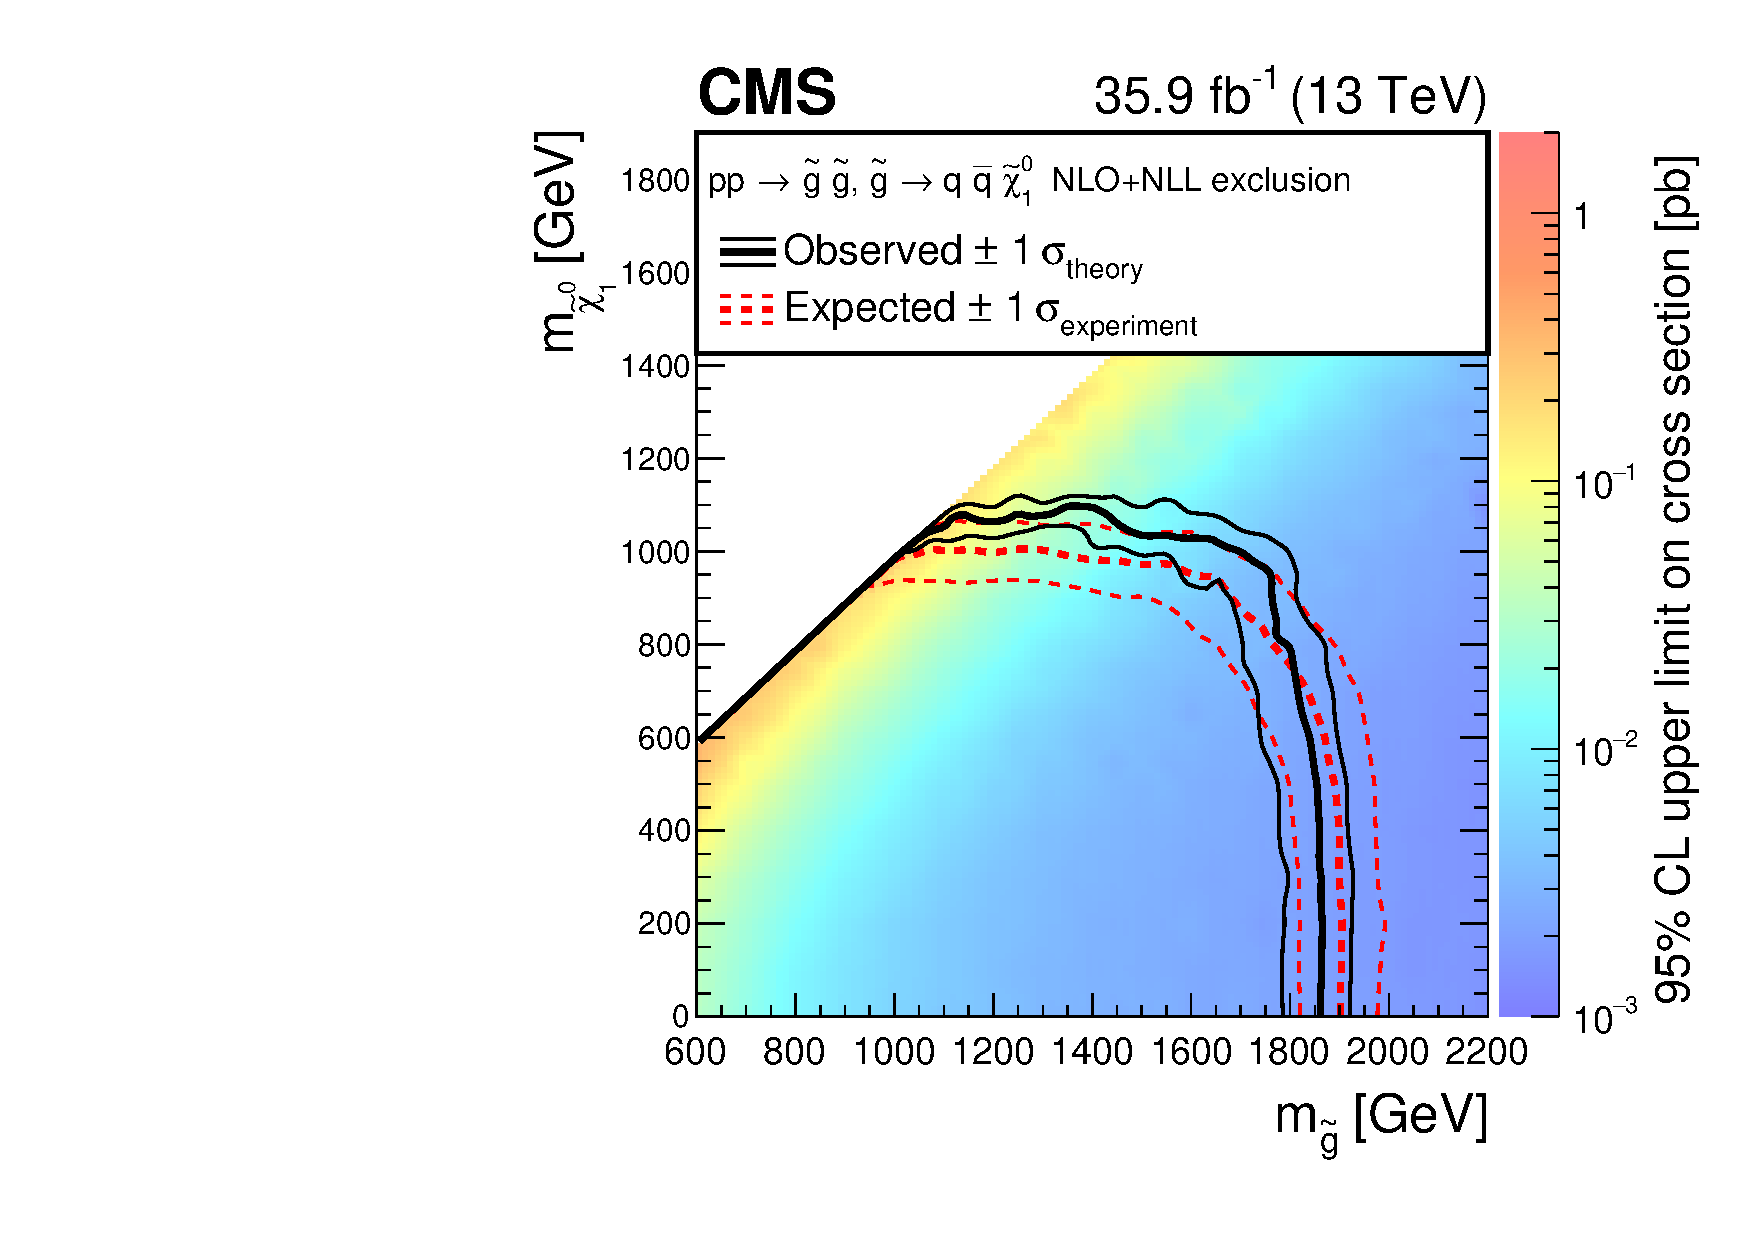
\includegraphics[width=0.45\textwidth]{results/figs/interpretations/T1qqqq_35p9ifb_Moriond2017_Mar07_XSEC}
	\caption{Exclusion limits at 95\% confidence level for gluino-mediated squark production of bottom (top left), top (top right), and light-flavor (bottom) squarks. The dashed red lines indicate the expected sensitivity and associated uncertainty, while the black lines indicate the observed exclusion limit and its associated theoretical uncertainty based on the signal cross-section.}
	\label{fig:limitsGluino}
\end{figure}
\begin{figure}
	\centering
	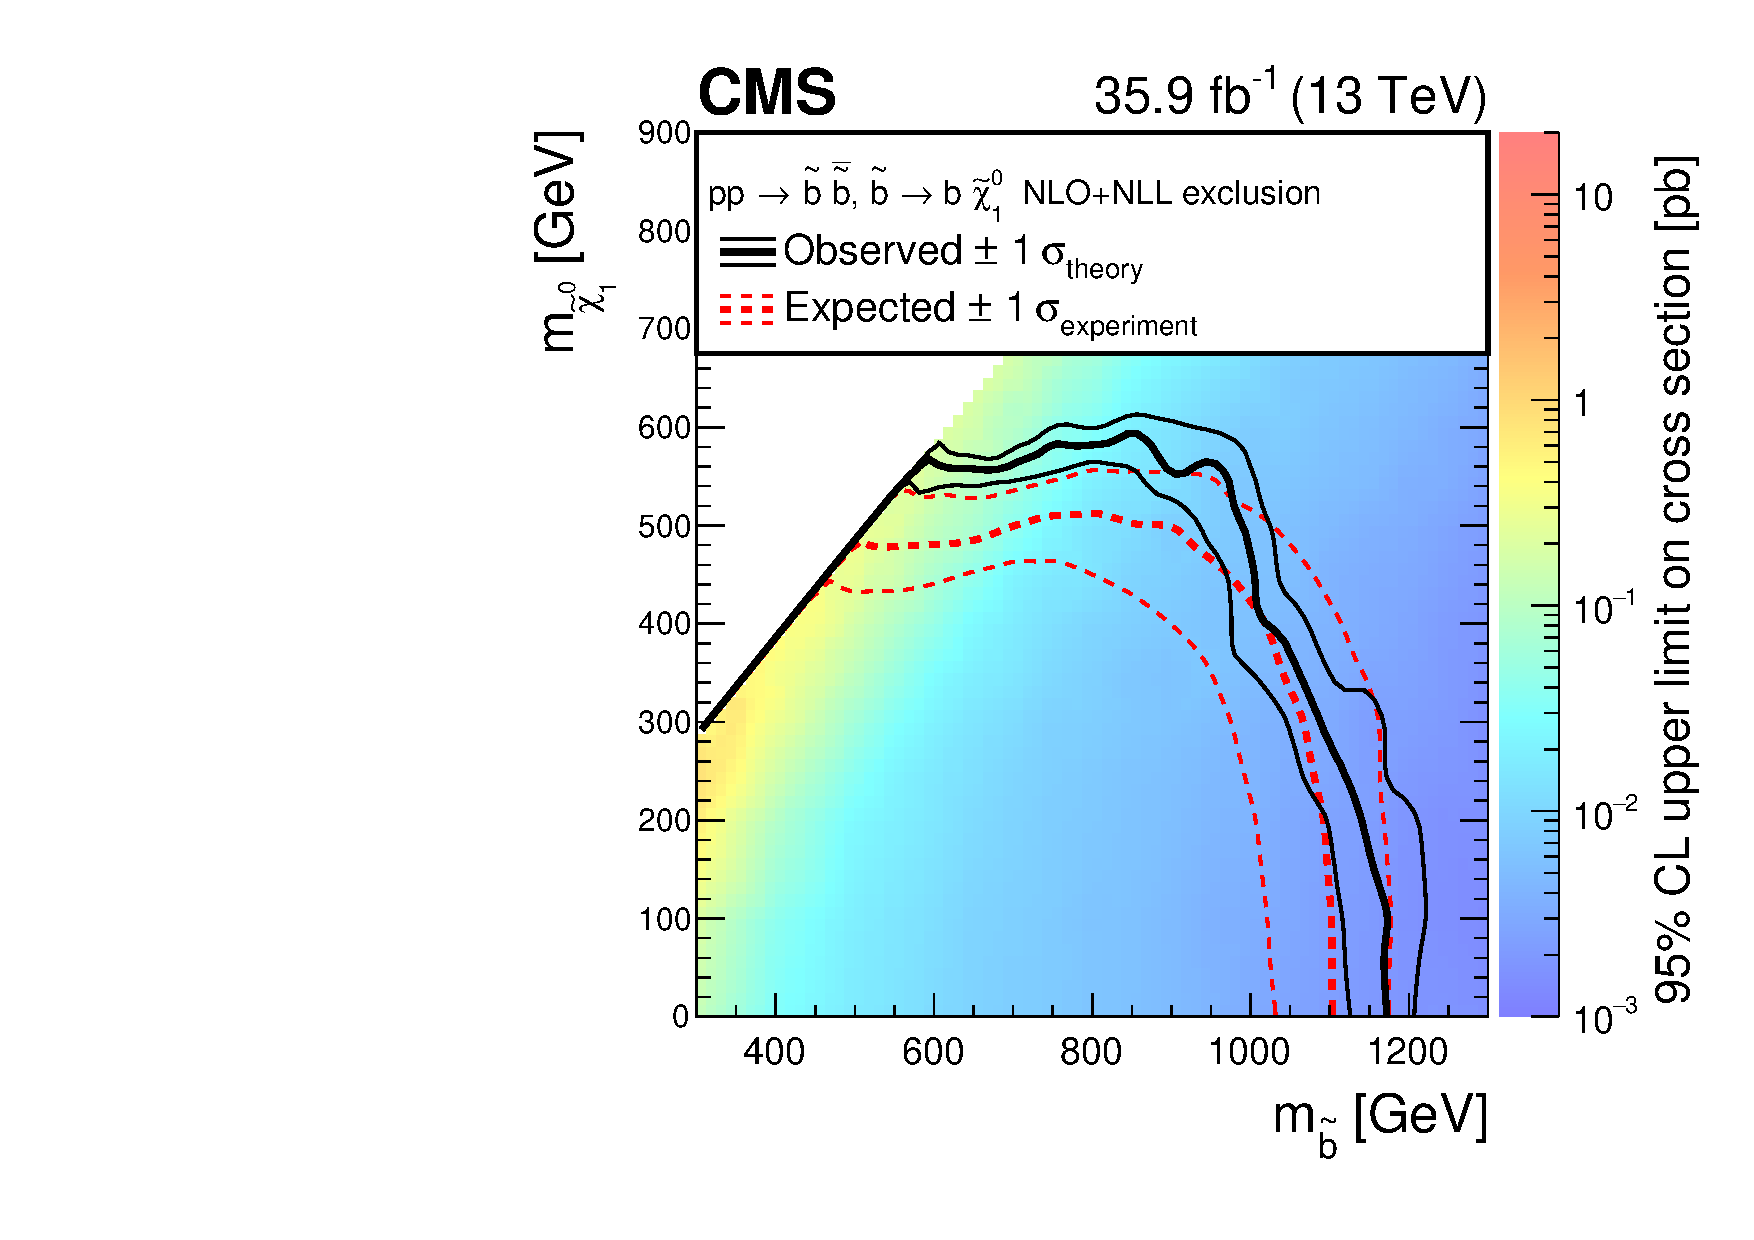
\includegraphics[width=0.45\textwidth]{results/figs/interpretations/T2bb_35p9ifb_Moriond2017_Mar07_XSEC}
	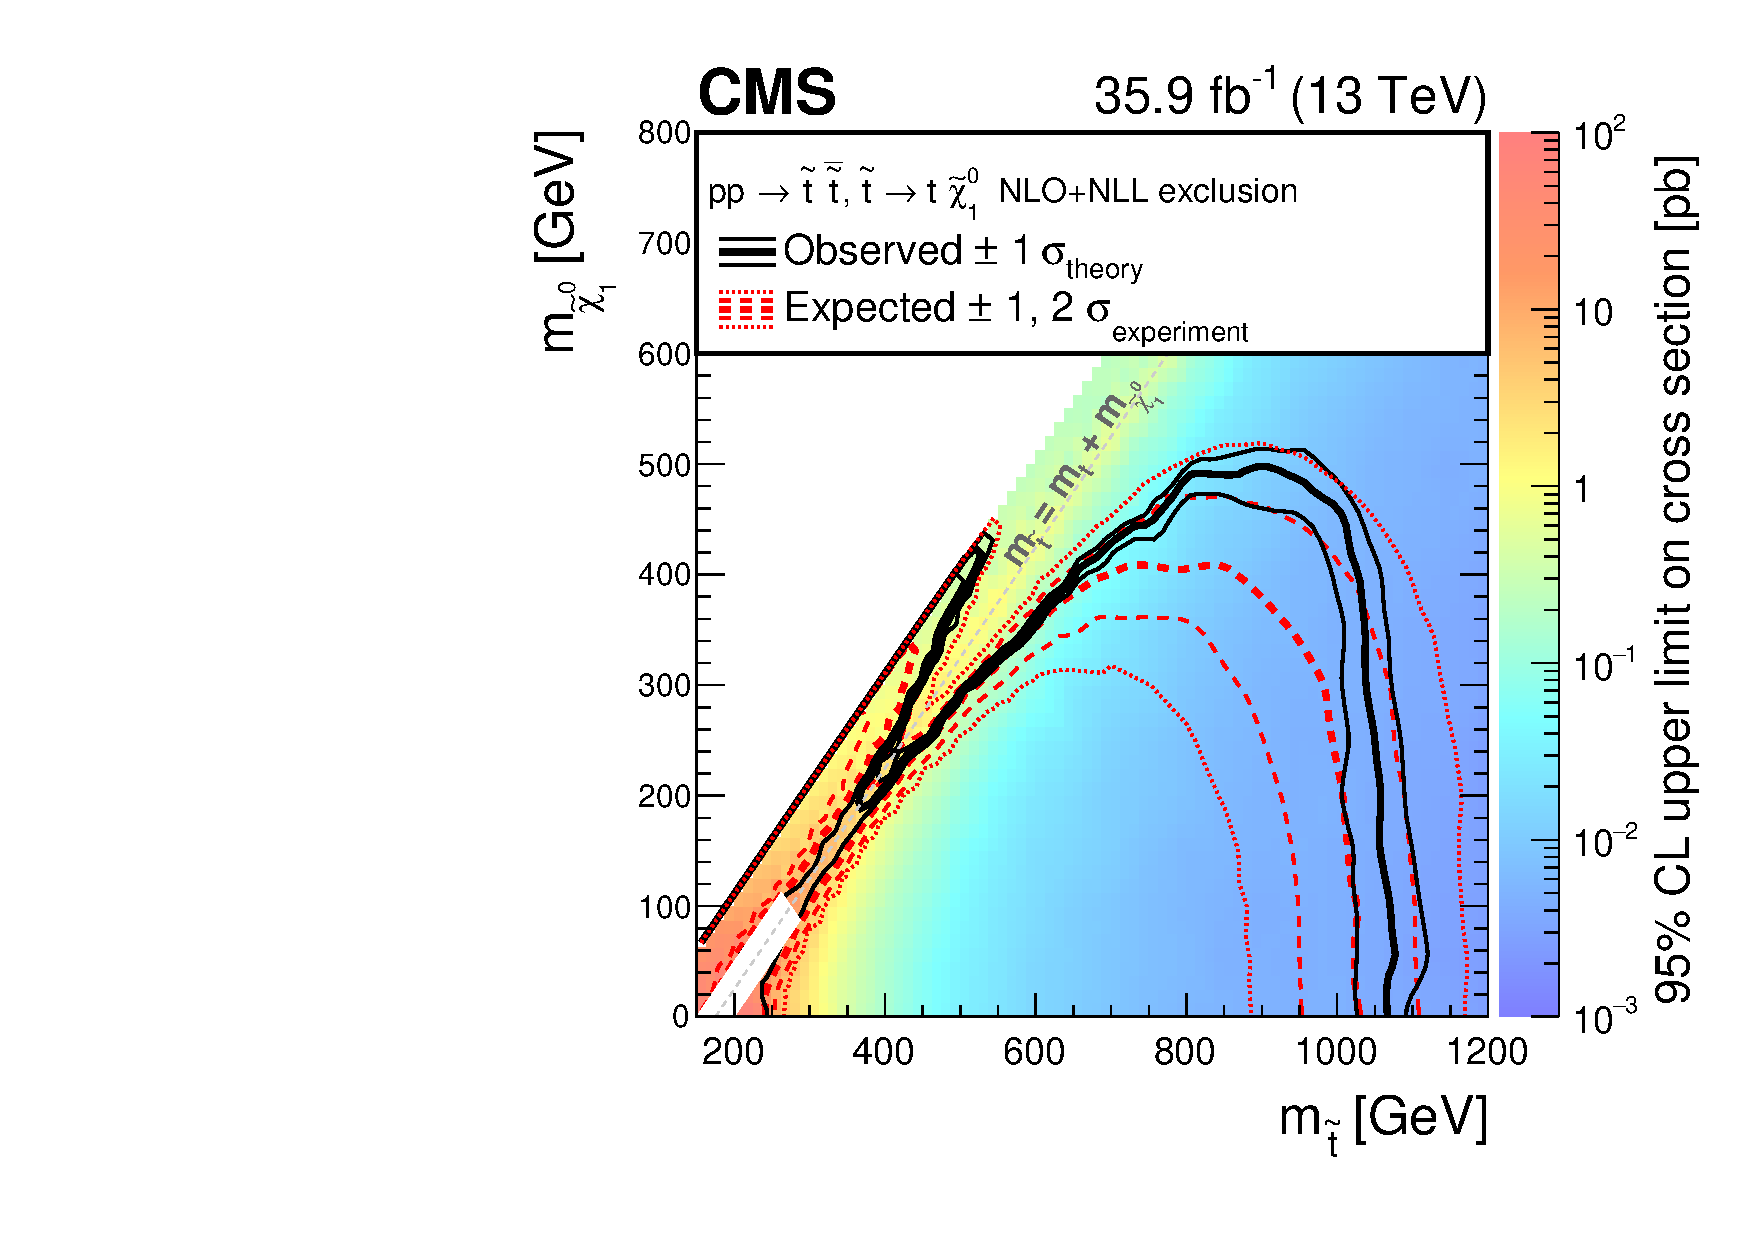
\includegraphics[width=0.45\textwidth]{results/figs/interpretations/T2tt_35p9ifb_Moriond2017_Mar07_XSEC}
	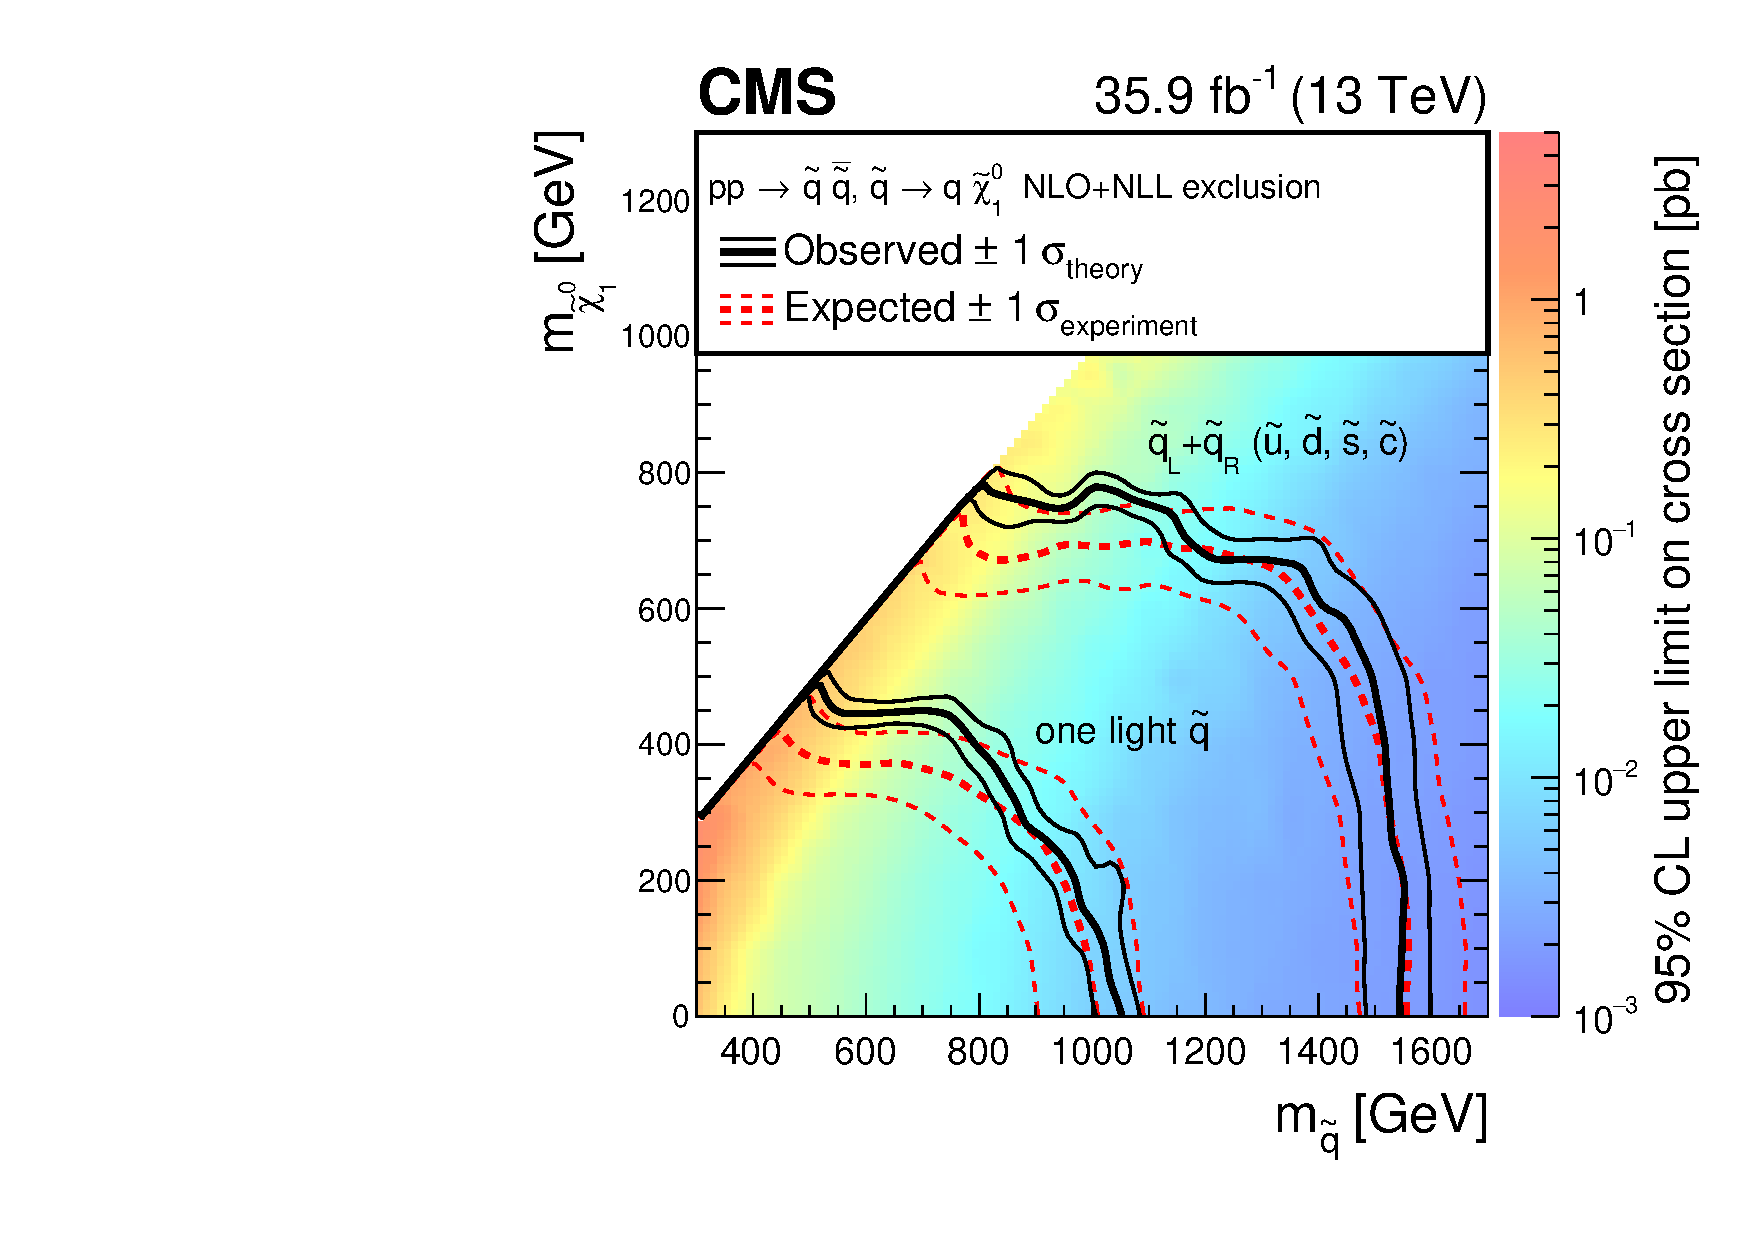
\includegraphics[width=0.45\textwidth]{results/figs/interpretations/T2qq_35p9ifb_Moriond2017_Mar07_XSEC}
	\caption{Exclusion limits at 95\% confidence level for direct squark production of bottom (top left), top (top right), and light-flavor (bottom) squarks. The dashed red lines indicate the expected sensitivity and associated uncertainty, while the black lines indicate the observed exclusion limit and its associated theoretical uncertainty based on the signal cross-section.}
	\label{fig:limitsSquark}
\end{figure}
\begin{figure}
	\centering
	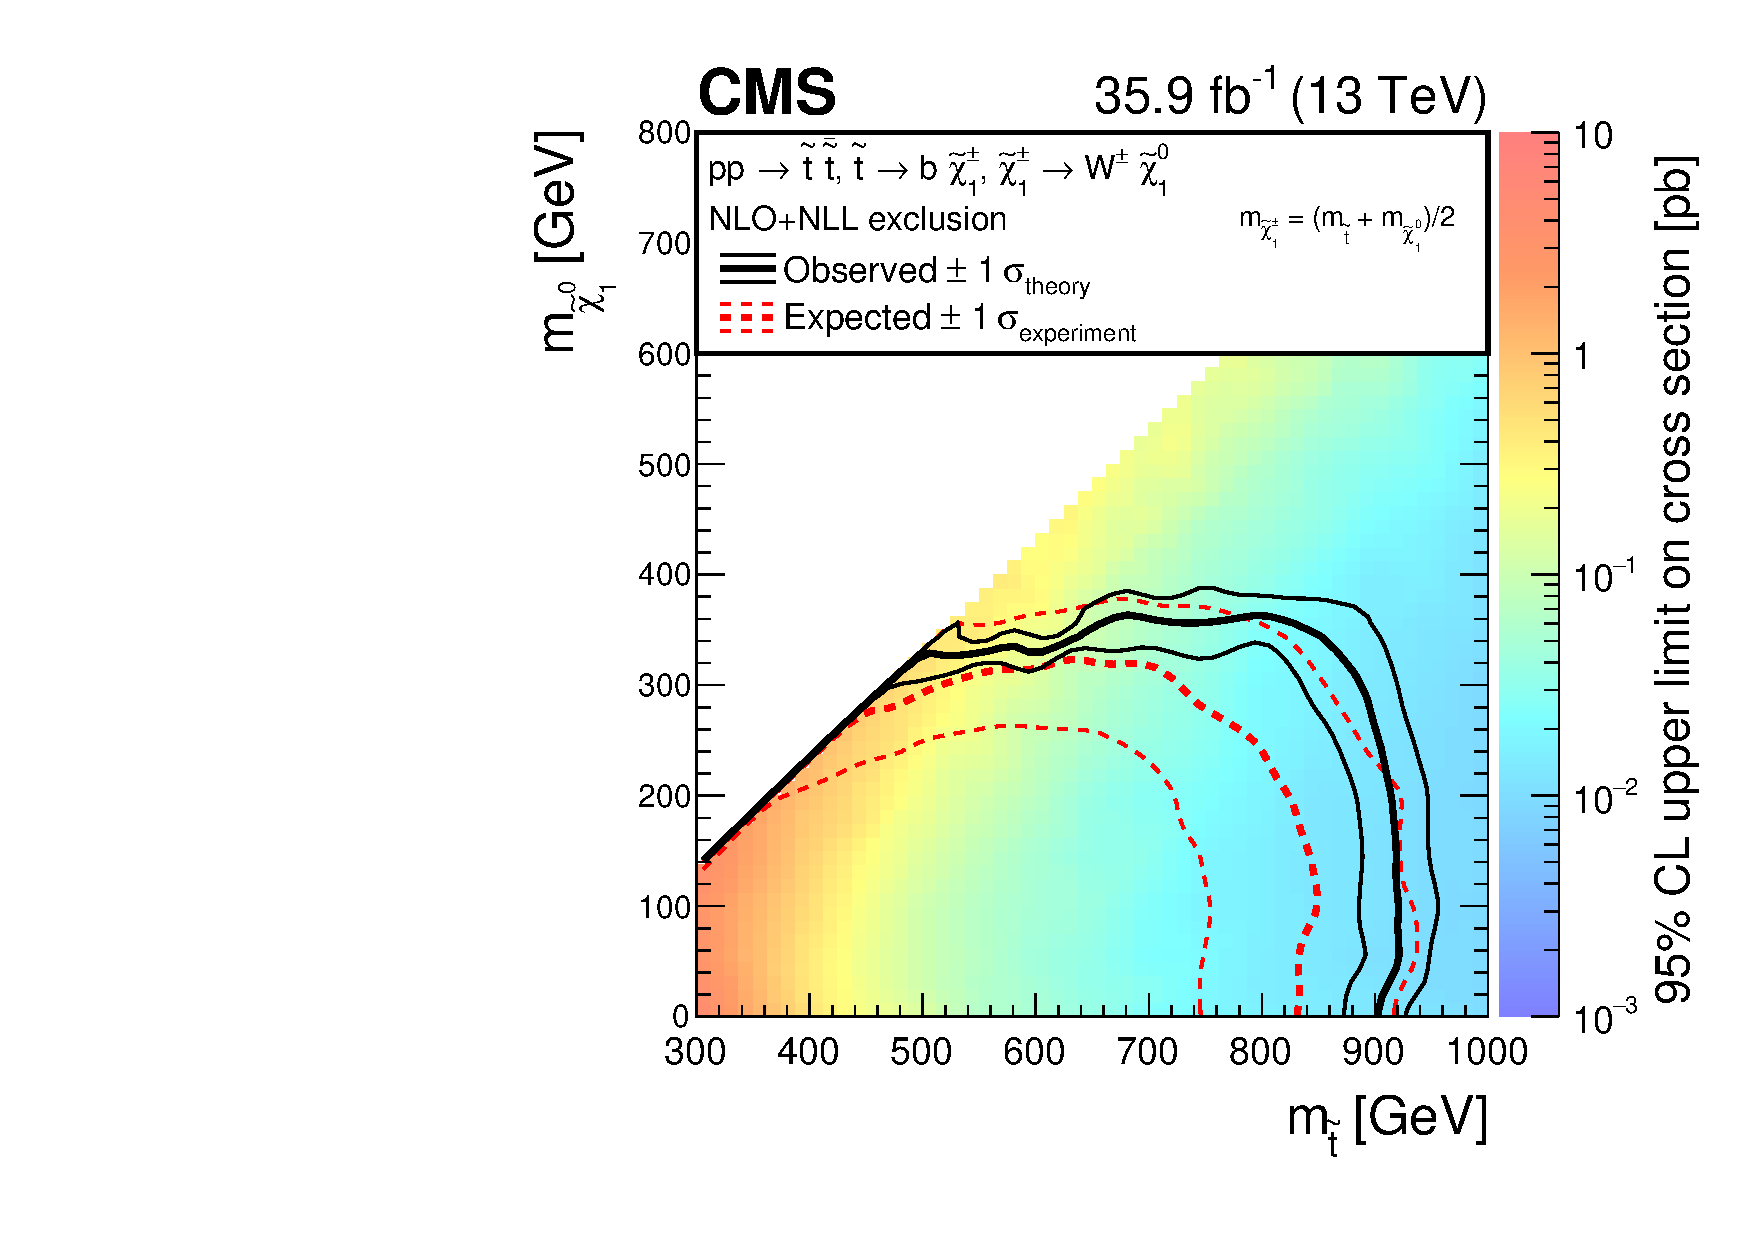
\includegraphics[width=0.45\textwidth]{results/figs/interpretations/T2bW_35p9ifb_Moriond2017_Mar07_XSEC}
	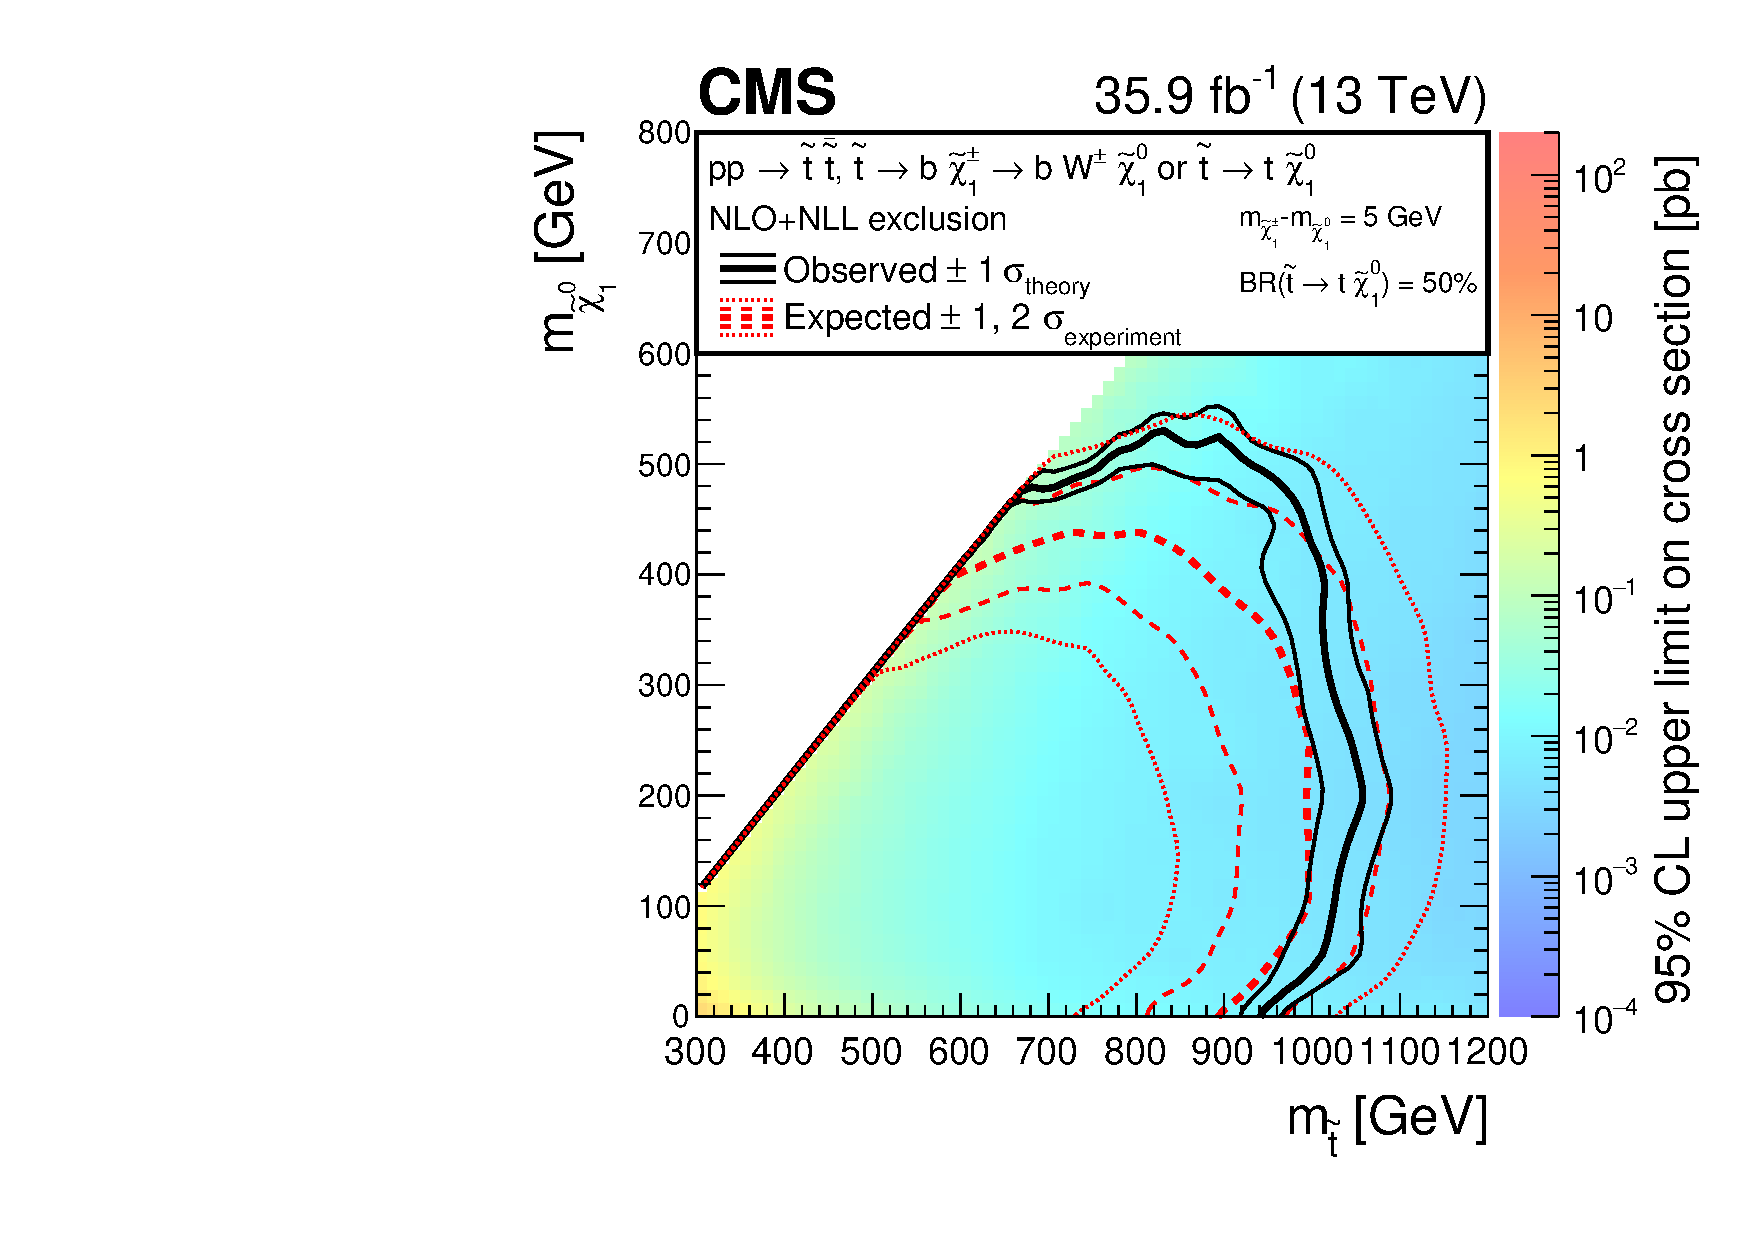
\includegraphics[width=0.45\textwidth]{results/figs/interpretations/T2bt_35p9ifb_Moriond2017_Mar07_XSEC}
	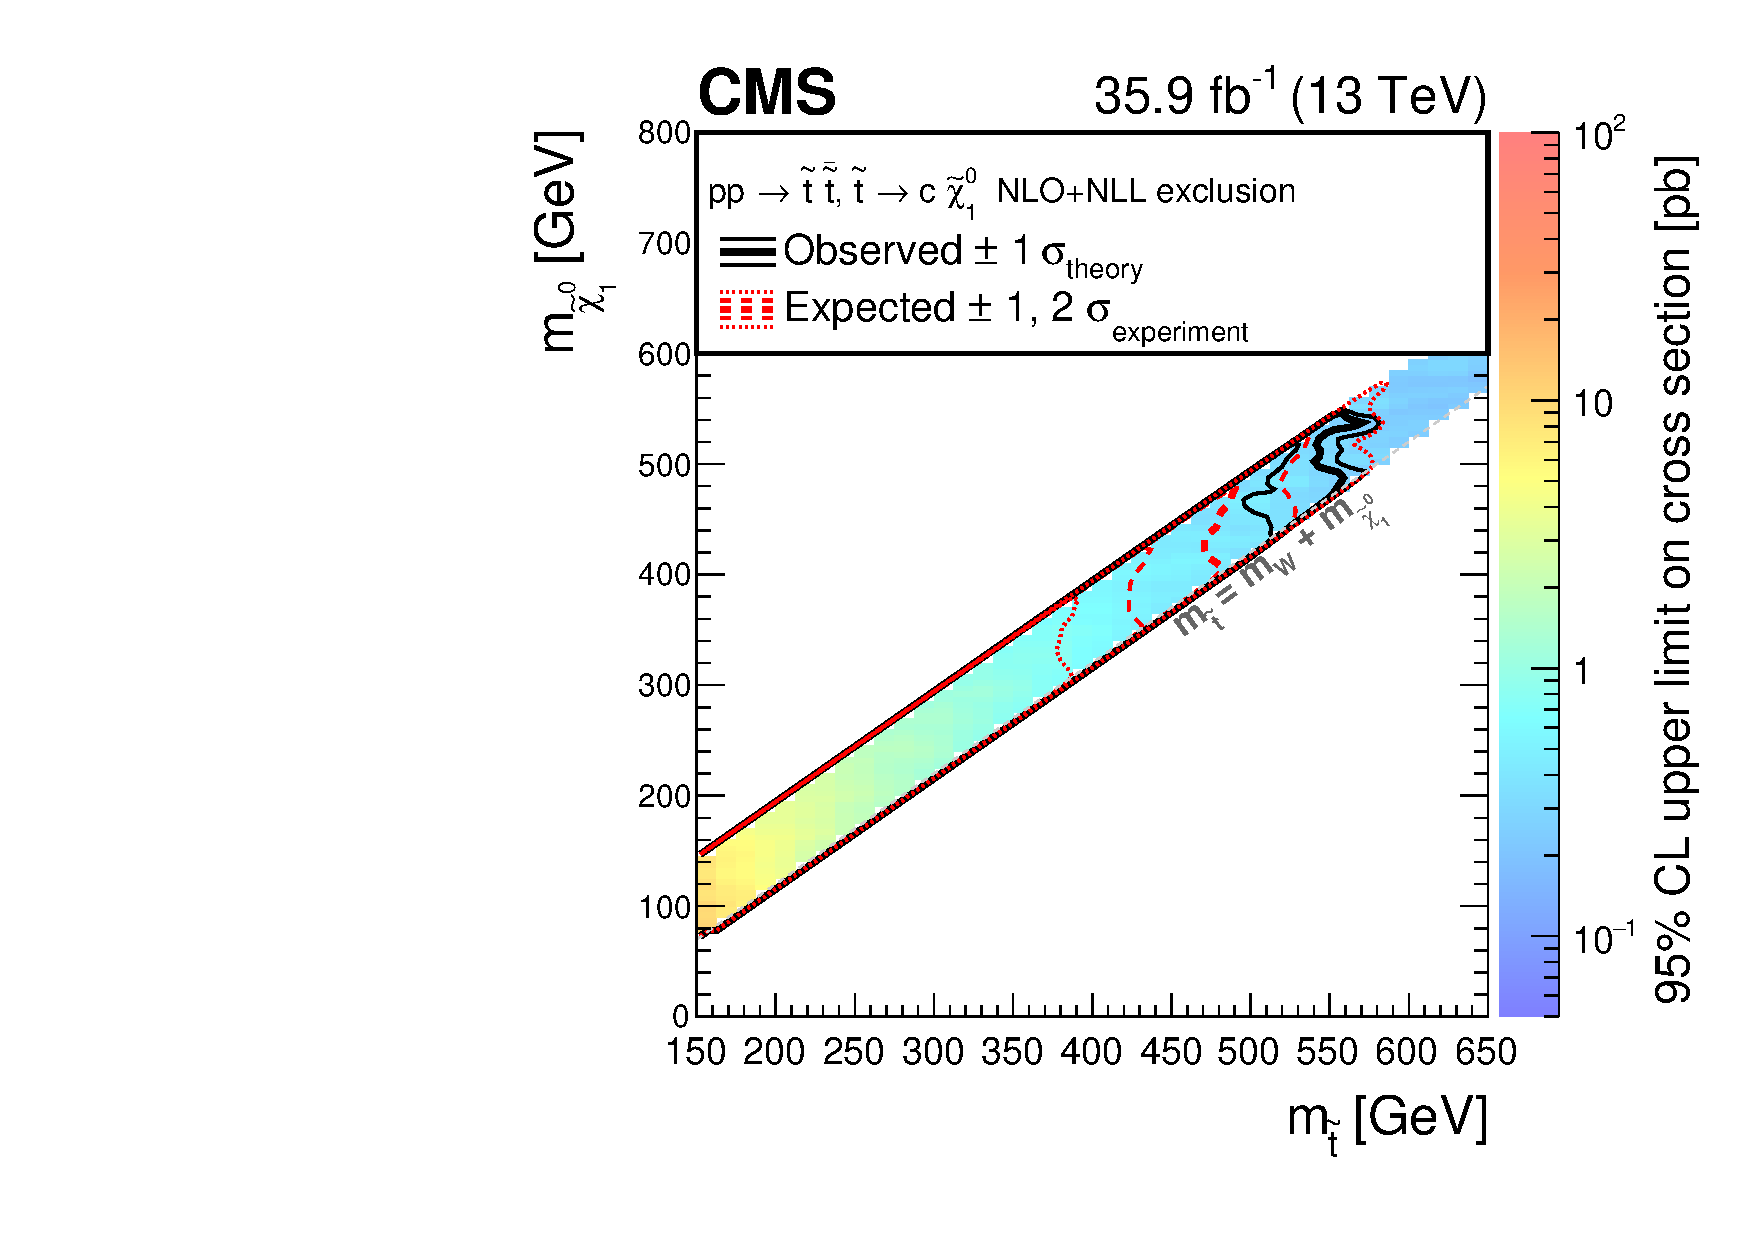
\includegraphics[width=0.45\textwidth]{results/figs/interpretations/T2cc_35p9ifb_Moriond2017_Mar07_XSEC}
	\caption{Exclusion limits at 95\% confidence level for direct top squark production In different decay modes. The top squark may decay through charginos (top left), where the chargino mass is taken as halfway-between the top squark and neutralino; a mixed scenario through charginos and neutralinos (top right), where the chargino mass is fixed to 5\GeV above the neutralino mass; or a compressed scenario, where the top squark is kinematically constrained to decay to charm quarks (bottom). The dashed red lines indicate the expected sensitivity and associated uncertainty, while the black lines indicate the observed exclusion limit and its associated theoretical uncertainty based on the signal cross-section.}
	\label{fig:limitsStop}
\end{figure}

\begin{table}
	\centering
	\begin{tabular}[]{l c r}
		\fm{Summary table of masses excluded} 
	\end{tabular}
	\caption{Summary of 95\% CL exclusion limits on the masses of SUSY particles (sparticles) produced by various simplified models. The limit on the produced sparticle is listed for a massless \lsp, along with the greatest excluded mass of \lsp for any mass of produced sparticle.}
	\label{tbl:limits}
\end{table}

% --------------------------------------------------------------------------- %
% --------------------------------------------------------------------------- %
